\chapter{Penalized and sparse multivariate regression}
\minitoc


\section{Ridge regression}
\subsection{Ridge estimator}
In the case where $X^\top X$ is singular (resp. has eigenvalues close to zero), the least squares estimate cannot be computed (resp. is not robust). A common approach to control the estimator variance is to solve the surrogate Ridge regression problem:
\[
\widehat \param^{\mathrm{ridge}}_{n,\lambda}\in  \argmin_{\param\in\rset^d}  \left\{\frac{1}{n}\|Y - X\param\|_2^2 + \lambda\|\param\|_2^2\right\}\eqsp,
\]
where $\lambda>0$. 
\begin{remark}
The matrix $n^{-1}X^\top X + \lambda  \Id_d$ is definite positive for all $\lambda>0$ as for all $u\in\rset^d$,
\[
u^\top (n^{-1}X^\top X + \lambda \Id_d)u = n^{-1}\|Xu\|_2^2 + \lambda  \|u\|_2^2\eqsp,
\]
which is positive for all $u\neq 0$. This remark allows to obtain the following result.
\end{remark}

\begin{shaded}
\begin{proposition}
\label{prop:least:squares:ridge}
The unique solution to the Ridge regression problem is given by
\[
\widehat \param^{\mathrm{ridge}}_{n,\lambda} = \frac{1}{n}\left(\frac{1}{n}X^\top X + \lambda \Id_d\right)^{-1}X^\top Y\eqsp.
\] 
If for all $1\leqslant i \leqslant n$, $Y_i = X^\top_i \param_{\star} + \varepsilon_i$ for some unknown $\param_\star\in\rset^d$ where the $(\varepsilon_i)_{1\leqslant i\leqslant n}$ are i.i.d. centered random variables in $\rset$ with variance $\sigma_\star^2$, this estimator is biased and satisfies 
\begin{align*}
\bE[\widehat \param^{\mathrm{ridge}}_{n,\lambda} ] - \param_*&= - \lambda\left(\frac{1}{n}X^\top X + \lambda \Id_d\right)^{-1}\param_\star\eqsp,\\
\bV[\widehat \param^{\mathrm{ridge}}_{n,\lambda} ] &= \frac{\sigma_\star^{2}}{n}\left(\frac{1}{n}X^\top X + \lambda \Id_d\right)^{-2}\frac{1}{n}X^\top X\eqsp.
\end{align*}
\end{proposition}
\end{shaded}
\begin{proof}
The unique expression of $\widehat \param^{\mathrm{ridge}}_{n,\lambda} $ is obtained similarly as in the proof of Proposition~\ref{prop:least:squares:full:rank}. Then,
$$
\bE[\widehat \param^{\mathrm{ridge}}_{n,\lambda}] =  \frac{1}{n}\left (\frac{1}{n}X^\top X + \lambda  \Id_d \right)^{-1}X^\top \bE[Y] =  \frac{1}{n}\left(\frac{1}{n} X^\top X + \lambda  \Id_d\right )^{-1}X^\top X\param_\star \eqsp.
$$
As the matrix $n^{-1}X^\top X$ is symmetric and real,  $ n^{-1}X^\top X$ is diagonalizable and $n^{-1}X^\top X$, $n^{-1}X^\top X + \lambda I_d$ and $(n^{-1} X^\top X + \lambda I_d)^{-1}$, are diagonalizable in the same orthonormal basis. Then, there exists nonnegative eigenvalues $\lambda_1\geqslant \ldots \geqslant \lambda_d$ and orthonormal eigenvectors $u_1, \ldots u_d$ in $\rset^d$ such that $n^{-1} X^\top X = \sum_{i=1}^d \lambda_i u_i u_i^\top$ and $(n^{-1}X^\top X + \lambda I_d)^{-1} = \sum_{i=1}^d (\lambda_i + \lambda)^{-1}u_i u_i^\top$. Therefore, 
$$
\bE[\widehat \param^{\mathrm{ridge}}_{n,\lambda}] -\param_\star=  \sum_{i=1}^d \lambda_i(\lambda_i + \lambda)^{-1}u_i u_i^\top\param_\star -  \sum_{i=1}^d u_i u_i^\top\param_\star =  - \lambda  \sum_{i=1}^d (\lambda_i + \lambda)^{-1}u_i u_i^\top\param_\star = - \lambda\left(\frac{1}{n}X^\top X + \lambda \Id_d\right)^{-1}\param_\star\eqsp.
$$
Similarly,
$$
\bV[\widehat \param^{\mathrm{ridge}}_{n,\lambda}]  =  \frac{1}{n^2}\left(\frac{1}{n}X^\top X + \lambda \Id_d\right)^{-1}X^\top \bV[Y]X  \left(\frac{1}{n}X^\top X + \lambda \Id_d\right)^{-1} = \frac{\sigma_\star^{2}}{n^2}\left(\frac{1}{n}X^\top X + \lambda \Id_d\right)^{-1}X^\top X  \left(\frac{1}{n}X^\top X + \lambda \Id_d\right)^{-1}\eqsp.
$$
Therefore,
$$
\bV[\widehat \param^{\mathrm{ridge}}_{n,\lambda}]  =   \frac{\sigma_\star^{2}}{n}\left(\frac{1}{n}X^\top X + \lambda \Id_d\right)^{-2}\frac{1}{n}X^\top X\eqsp.
$$
\end{proof}
\begin{remark}
By Proposition~\ref{prop:least:squares:ridge}, 
$$
\bV[\widehat \param^{\mathrm{ridge}}_{n,\lambda}]  = \frac{\sigma_\star^{2}}{n^2}\left(\frac{1}{n}X^\top X + \lambda \Id_d\right)^{-1}X^\top X  \left(\frac{1}{n}X^\top X + \lambda \Id_d\right)^{-1}\eqsp.
$$
On the other hand, the variance of the full rank estimator is 
$$
\bV[\widehat \param^{}_{n}]  = \sigma_\star^{2}\left(X^\top X\right)^{-1}\eqsp.
$$
Therefore, writing $M_\lambda = (X^\top X + \lambda n \Id_d)^{-1}X^\top X$,
\begin{align*}
\bV[\widehat \param^{\mathrm{ridge}}_{n,\lambda}]  - \bV[\widehat \param^{}_{n}] & =  \frac{\sigma_\star^{2}}{n^2}\left(\frac{1}{n}X^\top X + \lambda \Id_d\right)^{-1}X^\top X  \left(\frac{1}{n}X^\top X + \lambda \Id_d\right)^{-1} - \sigma_\star^{2}\left(X^\top X\right)^{-1}\\
&= \sigma_\star^{2}\left(X^\top X + \lambda n \Id_d\right)^{-1}X^\top X  \left(X^\top X + \lambda n \Id_d\right)^{-1} - \sigma_\star^{2}\left(X^\top X\right)^{-1}\\
&= \sigma_\star^{2}M_\lambda \left(X^\top X\right)^{-1}M_\lambda^\top  - \sigma_\star^{2}\left(X^\top X\right)^{-1}\\
&= \sigma_\star^{2}M_\lambda\left((X^\top X)^{-1}  - M_\lambda^{-1}(X^\top X)^{-1}(M_\lambda^\top)^{-1}\right)M_\lambda^{\top}\\
&= -\sigma_\star^{2}M_\lambda\left(2n\lambda(X^\top X)^{-2} + (n\lambda)^2(X^\top X)^{-3}\right)M_\lambda^{\top}\\
&= -\sigma_\star^{2}(X^\top X + \lambda n \Id_d)^{-1}\left(2n\lambda\Id_d + (n\lambda)^2(X^\top X)^{-1}\right)(X^\top X + \lambda n \Id_d)^{-1}\eqsp.
\end{align*}
Therefore, the matrix $\bV[\widehat \param^{\mathrm{ridge}}_{n,\lambda}]  - \bV[\widehat \param^{}_{n}]$ is negative semi-definite i.e. $\bV[\widehat \param^{\mathrm{ridge}}_{n,\lambda}]\leqslant \bV[\widehat \param^{}_{n}]$.
\end{remark}

\begin{remark}
If $X$ is an orthonormal matrix, $X^\top X = \Id_d$ and
\begin{equation*}
\bV[\widehat \param^{\mathrm{ridge}}_{n,\lambda}]  = \frac{\sigma_\star^{2}}{n^2}\left(\frac{1}{n}X^\top X + \lambda \Id_d\right)^{-1}X^\top X  \left(\frac{1}{n}X^\top X + \lambda \Id_d\right)^{-1}= \frac{\sigma^2_\star}{(1+n\lambda)^2}\Id_d\eqsp.
\end{equation*}
\end{remark}

\subsection{Risk}
\begin{proposition}
\label{prop:risk:ridge}
Assume that for all $1\leqslant i \leqslant n$, $Y_i = X^\top_i \param_{\star} + \varepsilon_i$ for some unknown $\param_\star\in\rset^d$ where the $(\varepsilon_i)_{1\leqslant i\leqslant n}$ are i.i.d. centered random variables in $\rset$ with variance $\sigma_\star^2$. For all $\lambda>0$,
$$
\bE\left[\mathsf{R}(\widehat \param^{\mathrm{ridge}}_{n,\lambda}) - \mathsf{R}(\param_\star)\right] = \lambda^2\param_\star^\top\left(\frac{1}{n}X^\top X + \lambda \Id_d\right)^{-2} \frac{1}{n}X^\top X \param_\star +\frac{\sigma_\star^{2}}{n}\mathrm{Trace}\left((n^{-1}X^\top X)^2(n^{-1}X^\top X + \lambda \Id_d)^{-2}\right)\eqsp.
$$
\end{proposition}
\begin{proof}
Following the full-rank risk analysis given in Section~\ref{sec:risk:fullrank}, we have
\begin{multline*}
\bE\left[\mathsf{R}(\widehat \param^{\mathrm{ridge}}_{n,\lambda}) - \mathsf{R}(\param_\star)\right] \\
=\left(\param_\star-\bE\left[\widehat \param^{\mathrm{ridge}}_{n,\lambda}\right]\right)^\top \left(\frac{1}{n}X^\top X\right) \left(\param_\star-\bE\left[\widehat \param^{\mathrm{ridge}}_{n,\lambda}\right] \right) + \bE\left[ \left(\bE\left[\widehat \param^{\mathrm{ridge}}_{n,\lambda}\right] - \widehat \param^{\mathrm{ridge}}_{n,\lambda}\right)^\top \left(\frac{1}{n}X^\top X\right) \left(\bE\left[\widehat \param^{\mathrm{ridge}}_{n,\lambda}\right] - \widehat \param^{\mathrm{ridge}}_{n,\lambda}\right)\right]\eqsp.
\end{multline*}
By Proposition~\ref{prop:least:squares:ridge}, the bias term is given by
\begin{align*}
\left(\param_\star-\bE\left[\widehat \param^{\mathrm{ridge}}_{n,\lambda}\right]\right)^\top \left(\frac{1}{n}X^\top X\right) \left(\param_\star-\bE\left[\widehat \param^{\mathrm{ridge}}_{n,\lambda}\right] \right) &= \frac{\lambda^2}{n}\left(\left(\frac{1}{n}X^\top X + \lambda \Id_d\right)^{-1}\param_\star\right)^\top X^\top X  \left(\left(\frac{1}{n}X^\top X + \lambda \Id_d\right)^{-1}\param_\star\right)\eqsp,\\
&= \frac{\lambda^2}{n}\param_\star^\top\left(\frac{1}{n}X^\top X + \lambda \Id_d\right)^{-1} X^\top X \left(\frac{1}{n}X^\top X + \lambda \Id_d\right)^{-1}\param_\star\eqsp,\\
&= \lambda^2\param_\star^\top\left(\frac{1}{n}X^\top X + \lambda \Id_d\right)^{-2} \frac{1}{n}X^\top X \param_\star\eqsp.
\end{align*}
By Lemma~\ref{ref:expectation:quadratic:trasform} and  Proposition~\ref{prop:least:squares:ridge}, the variance term is given by
\begin{align*}
\bE\left[ \left(\bE\left[\widehat \param^{\mathrm{ridge}}_{n,\lambda}\right] - \widehat \param^{\mathrm{ridge}}_{n,\lambda}\right)^\top \left(\frac{1}{n}X^\top X\right) \left(\bE\left[\widehat \param^{\mathrm{ridge}}_{n,\lambda}\right] - \widehat \param^{\mathrm{ridge}}_{n,\lambda}\right)\right] &= \mathrm{Trace}\left(\frac{1}{n}X^\top X \bV[\widehat \param^{\mathrm{ridge}}_{n,\lambda}]\right)\eqsp,\\
&= \frac{\sigma_\star^{2}}{n}\mathrm{Trace}\left(\frac{1}{n}X^\top X\left(\frac{1}{n}X^\top X + \lambda \Id_d\right)^{-2}\frac{1}{n}X^\top X\right)\eqsp,\\
&= \frac{\sigma_\star^{2}}{n}\mathrm{Trace}\left((n^{-1}X^\top X)^2(n^{-1}X^\top X + \lambda \Id_d)^{-2}\right)\eqsp,
\end{align*}
which concludes the proof.
\end{proof}
\begin{remark}
\begin{itemize}
\item The bias term increases with $\lambda$. It is 0 when $\lambda = 0$ and it converges to $\param_\star^\top X^\top X\param_\star / n$ when $\lambda\to \infty$.
\item  The variance term decreases with $\lambda$. It is $\sigma_\star^2 d /n$ when $\lambda = 0$ and it converges to $0$ when $\lambda\to \infty$.
\item The mean square error of the estimator is then given by
\[
\bE\left[\left\|\widehat \param^{\mathrm{ridge}}_{n,\lambda}-\param_*\right\|_2^2\right] = \mathrm{Trace}\left(\bV[\widehat \param^{\mathrm{ridge}}_{n,\lambda}]\right) + \left\|\bE[\widehat \param^{\mathrm{ridge}}_{n,\lambda}] - \param_*\right\|_2^2\eqsp.
\]
Let $(\vartheta_1,\ldots,\vartheta_d)$ be an orthonormal basis of $\rset^d$ of eigenvectors of $X^\top X$ associated with the eigenvalues $(\lambda_1,\ldots,\lambda_d)\in\rset^d$. Then,
\[
\bE\left[\left\|\widehat \param^{\mathrm{ridge}}_{n,\lambda}-\param_*\right\|_2^2\right] =  \sigma_\star^2 \sum_{j=1}^d \frac{\lambda_j}{(\lambda_j+\lambda)^2} + \lambda^2  \sum_{j=1}^d \frac{\langle \param_* \eqsp; \vartheta_j\eqsp\rangle^2}{(\lambda_j+\lambda)^2}\eqsp.
\]
The mean square error is therefore a sum of two contributions, a bias related term which increases with $\lambda$ and a variance related term which decreases with $\lambda$. In practice, the value of $\lambda$ is chosen using cross-validation.
\end{itemize}
\end{remark}
Using the risk analysis for the Ridge-based estimator, we can tune the regularization parameter $\lambda$ to obtain
a  better bound than the $\sigma_\star^2 d /n$ bound of the case $\lambda = 0$.

\begin{proposition}
Choosing $\lambda = \lambda_\star$ where 
$$
\lambda_\star = \frac{\sigma_\star \mathrm{Trace}\left(X^\top X\right)^{1/2}}{\sqrt{n}\|\param_\star\|_2} \eqsp.
$$
yields
$$
\bE\left[\mathsf{R}(\widehat \param^{\mathrm{ridge}}_{n,\lambda_\star}) - \mathsf{R}(\param_\star)\right]  \leqslant \frac{\sigma_\star \|\param_\star\|_2 \mathrm{Trace}\left(X^\top X\right)^{1/2}}{\sqrt{n}}  \eqsp.
$$
\end{proposition}
\begin{proof}
Let $(\vartheta_1,\ldots,\vartheta_d)$ be an orthonormal basis of $\rset^d$ of eigenvectors of $n^{-1}X^\top X$ associated with the eigenvalues $(\lambda_1,\ldots,\lambda_d)\in\rset^d$. Therefore,
$$
 \lambda^2\param_\star^\top\left(\frac{1}{n}X^\top X + \lambda I_d\right)^{-2} \frac{1}{n}X^\top X \param_\star = \lambda\sum_{i=1}^d \param_\star^\top \frac{\lambda \lambda_i}{(\lambda_i + \lambda)^2} u_iu_i^\top \param_\star \leqslant  \frac{\lambda}{2}\|\param_\star\|_2^2\eqsp,
$$
since for all $1\leqslant i \leqslant d$, $2\lambda \lambda_i \leqslant (\lambda + \lambda_i)^2$ implies $\lambda \lambda_i/(\lambda + \lambda_i)^2 \leqslant 1/2$. On the other hand,
$$
\frac{\sigma_\star^{2}}{n}\mathrm{Trace}\left((n^{-1}X^\top X)^2(n^{-1}X^\top X + \lambda I_d)^{-2}\right) = \frac{\sigma_\star^{2}}{n}\mathrm{Trace}\left(n^{-1}X^\top X\sum_{i=1}^d\frac{\lambda_i}{(\lambda + \lambda_i)^2}u_iu_i^\top\right) \leqslant \frac{\sigma_\star^{2}}{2n\lambda }\mathrm{Trace}\left(n^{-1}X^\top X\right) \eqsp.
$$
Therefore, by Proposition~\ref{prop:risk:ridge},
$$
\bE\left[\mathsf{R}(\widehat \param^{\mathrm{ridge}}_n) - \mathsf{R}(\param_\star)\right]  \leqslant \frac{\lambda}{2}\|\param_\star\|_2^2 + \frac{\sigma_\star^{2}}{2n\lambda}\mathrm{Trace}\left(n^{-1}X^\top X\right)\eqsp.
$$
The upper-bound is then minimized by choosing 
$$
\lambda_\star = \frac{\sigma_\star \mathrm{Trace}\left(X^\top X\right)^{1/2}}{\sqrt{n}\|\param_\star\|_2} \eqsp.
$$
\end{proof}

\subsection{Choice of $\lambda$}
\label{sec:ridge:choicepen}
Information-based metrics such as Akaike Information Criterion (AIC, \cite{akaike1974new}) or Bayesian Information Criterion (BIC, \cite{schwarz1978estimating}) are popular approaches to select $\lambda$ in practical applications to balance between accuracy and complexity. On the other hand cross-validation techniques are widely used in machine learning and foster models with good prediction performance.

A standard approach is to use a $K$-fold cross-validation to split data between train and test subsets. The dataset $\mathcal{D} = \{(X_i,Y_i)\}_{1\leq i\leq n}$ is randomly divided into a partition made of $K$ subsets approximately equally sized $\mathcal{D}_1, \ldots \mathcal{D}_K$. For all $1\leqslant k \leqslant K$, let $n_k$ be the number of couples $(X_i,Y_i)$ in $\mathcal{D}_k$. For all $1\leqslant k \leqslant K$, write $\bf X_k$ (resp. $\bf X_{-k}$) the matrix containing all input features $X_i$, $1\leqslant i\leqslant n$, such that $(X_i,Y_i)\in \mathcal{D}_k$ (resp. containing all input features $X_i$, $1\leqslant i\leqslant n$, such that $(X_i,Y_i)\notin \mathcal{D}_k$). Similarly, write $\bf Y_k$ (resp. $\bf Y_{-k}$) the vector containing all observations $Y_i$, $1\leqslant i\leqslant n$, such that $(X_i,Y_i)\in \mathcal{D}_k$ (resp. containing all observations $Y_i$, $1\leqslant i\leqslant n$, such that $(X_i,Y_i)\notin \mathcal{D}_k$). To assess the predictive performance of a model, we choose a loss function, and for each model, the model is trained $K$ times using successively $\bf X_{-k}$ and $\bf Y_{-k}$, $1\leqslant k\leqslant K$, to estimate the parameters of the model and $\bf X_{k}$ and $\bf Y_{k}$ to compute the loss function, i.e each model is associated with $K$ predictive scores computed on a dataset which was not used to train the model. Usually, the model with best average score on the test sets is chosen (but considering the empirical variance of the test scores is also interesting). An example of the procedure is displayed in Algorithm~\ref{alg:cv:ridge}.

There exist many ways to build the different groups of samples. In Leave One Out (LOO) strategies,  training  sets are created using all samples except one $\{(X_i,Y_i)\}_{1\leqslant i\neq i_*\leqslant n}$, the test score being being evaluated only with $(X_{i_*},Y_{i_*})$. 

Cross-validation can be performed using Scikit-learn and its ridge regression with built-in cross-validation, see for instance \url{https://scikit-learn.org/dev/modules/generated/sklearn.linear\_model.RidgeCV.html}. Figure~\ref{fig:cv:grid} illustrate a way data can be split to perform a cross-validation\footnote{\url{https://scikit-learn.org/stable/modules/cross\_validation.html}}.

\begin{figure}
\label{fig:cv:grid}
\begin{center}
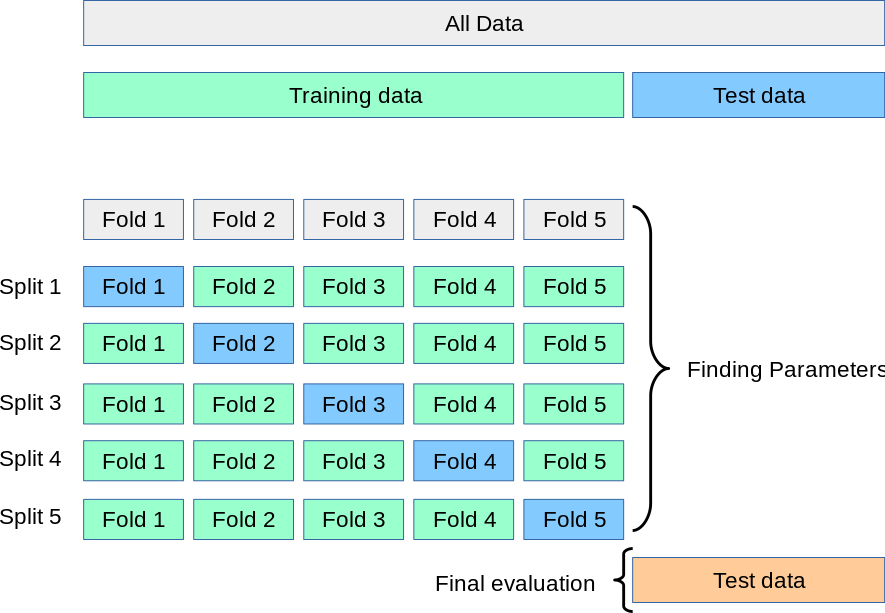
\includegraphics[width = .7\linewidth]{./Illustrations/grid_search_cross_validation}
\end{center}
\caption{An illustration on how to split data to select hyperparameters using $K$-fold cross-validation, see \url{https://scikit-learn.org/stable/modules/cross\_validation.html}.}
\end{figure}



\begin{algorithm}
\caption{K-fold cross-validation to select $\lambda$}\label{alg:cv:ridge}
\begin{algorithmic}
\Require $K$, $\mathcal{D}_1, \ldots \mathcal{D}_K$, candidate values $\{\lambda_1,\ldots,\lambda_p\}$, $p\geqslant 1$.
\For{$j\in\{1,\ldots,p\}$}
\For{$k\in\{1,\ldots,K\}$}
    \State Compute
$$
\widehat \param^{\mathrm{ridge}}_{n,k,\lambda_j} = \frac{1}{n-n_k}\left(\frac{1}{n-n_k}\bf{Y}_{-k}^\top \bf{Y}_{-k} + \lambda \Id_d\right)^{-1}\bf{Y}_{-k}^\top \bf{Y}_{-k}\eqsp.
$$
    \State Compute
$$
\mathcal{L}_k(\lambda_j) = \left\|\bf{Y}_k - \bf{X}_k \widehat \param^{\mathrm{ridge}}_{n,k,\lambda_j}\right\|_2^2\eqsp.
$$ 
\EndFor
\State Set
$$
\overline{\mathcal{L}}(\lambda_j) = \frac{1}{K}\sum_{k=1}^{K}\mathcal{L}_k(\lambda_j)\eqsp.
$$
\EndFor
\State Set
$$
\widehat \lambda = \mathrm{Argmin}_{\lambda_1,\ldots\lambda_p}\overline{\mathcal{L}}(\lambda)\eqsp.
$$
\end{algorithmic}
\end{algorithm}
\begin{figure}
\begin{center}
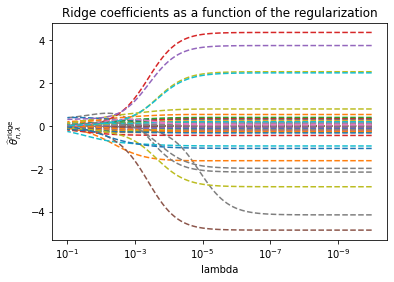
\includegraphics[width = .7\linewidth]{./Illustrations/ridge_coef.png}
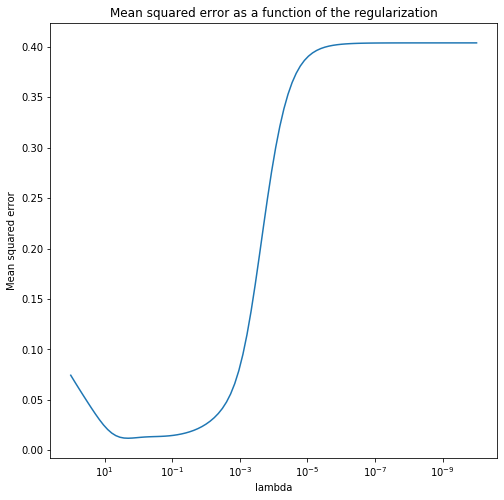
\includegraphics[width = .7\linewidth]{./Illustrations/ridge_rmse_test.png}
\end{center}
\caption{Ridge regression is used to predict the Brazilian inflation based on many observed variables, see \url{https://github.com/gabrielrvsc/HDeconometrics/}. The model is trained using $n=140$ data with for each $1\leqslant i \leqslant n$, $X_i\in\rset^{93}$, i.e. $d  =93$. The features are econometric data available each month. (Top) Estimated coefficient $\widehat \param^{\mathrm{ridge}}_{n,\lambda}$ as a function of $\lambda$. (Bottom) Mean squared error between the true observations and the predictions over the test set with $15$ new data points.}
\end{figure}


\begin{figure}
\begin{center}
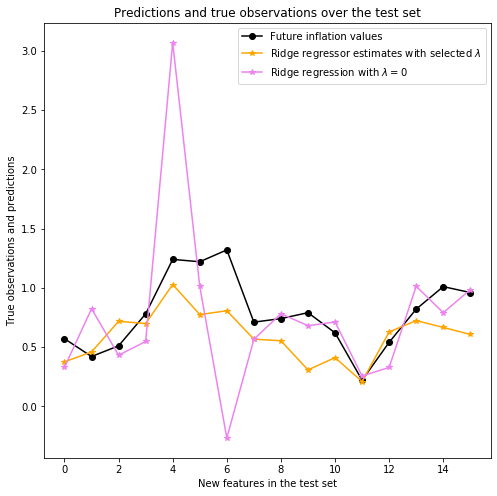
\includegraphics[width = .7\linewidth]{./Illustrations/ridge_pred_inflation.png}
\end{center}
\caption{Ridge regression is used to predict the Brazilian inflation based on many observed variables, see \url{https://github.com/gabrielrvsc/HDeconometrics/}. The model is trained using $n=140$ data with for each $1\leqslant i \leqslant n$, $X_i\in\rset^{93}$, i.e. $d  =93$. The features are econometric data available each month. In this experiment, 15 new data points in a test set are used to evaluate the Ridge estimator. We present an ordinary least squares estimate (i.e with $\lambda = 0$) and the estimate obtained by selecting $\lambda$ with a leave-one-out Cross-Validation. The MSE on the test set are 0.016 for the cross-validated $\lambda$ and 0.398 for $\lambda = 0$.}
\end{figure}



%%%%%%%%%%%%%%%%%%%%%%%%%%%%%%%%%%%%%
%%%%%%%%%%%%%%%%%%%%%%%%%%%%%%%%%%%%%


\section{Lasso regression}
The Least Absolute Shrinkage and Selection Operator (Lasso) regression, introduced in \cite{tibshirani1996regression}, is a $\mathrm{L}_1$ based regularized regression which aims at fostering sparsity. The objective is to solve the following minimization problem,
\begin{equation}
\label{eq:lasso:obj}
\widehat \param^{\mathrm{lasso}}_{\lambda,n}\in  \argmin_{\param\in\rset^d}  \left\{\frac{1}{n}\|Y - X\param\|_2^2 + \lambda\|\param\|_1\right\}\eqsp,
\end{equation}
where $\lambda>0$ and
\[
\|\param\|_1 = \sum_{j=1}^d|\param_j|\eqsp.
\]
The function $\param \mapsto n^{-1}\|Y - X\param\|_2^2 + \lambda\|\param\|_1$ is convex but not differentiable and the solution to this problem may  not be unique. This approach shrinks some coefficients of $\param$ and sets others to 0. The objective is to balance the impact of feature selection and regularization.  By Lemma~\ref{lem:lasso:loss}, even when the Lasso solution is not unique, the solutions to \eqref{eq:lasso:obj} share some properties. 

\begin{lemma}[\cite{tibshirani2013lasso}]
\label{lem:lasso:loss}
For all $\lambda>0$, $n\geqslant 1$, all solutions $\widehat \param^{\mathrm{lasso}}_{\lambda,n}$ to \eqref{eq:lasso:obj} have the same fitted value $X \widehat \param^{\mathrm{lasso}}_{\lambda,n}$ and the same $\mathrm{L}_1$-norm $\|\widehat \param^{\mathrm{lasso}}_{\lambda,n}\|_1$.
\end{lemma}

\begin{proof}
\begin{itemize}
\item Let $\widehat \param^{\mathrm{lasso}}_{1,\lambda,n}$ and $\widehat \param^{\mathrm{lasso}}_{2,\lambda,n}$ be two solutions of \eqref{eq:lasso:obj}. Assume that $X\param^{\mathrm{lasso}}_{1,\lambda,n} \neq X\param^{\mathrm{lasso}}_{2,\lambda,n}$. Then, for all $\gamma\in(0,1)$, writing $\param^{\mathrm{lasso}}_{\gamma,\lambda,n} = \gamma \param^{\mathrm{lasso}}_{1,\lambda,n} + (1-\gamma)\param^{\mathrm{lasso}}_{2,\lambda,n}$ and since $\|\cdot\|_2^2$ is stricly convex, 
$$
\|Y - X\param^{\mathrm{lasso}}_{\gamma,\lambda,n}\|^2_2 = \|\gamma(Y - X\param^{\mathrm{lasso}}_{1,\lambda,n}) + (1-\gamma)(Y - X\param^{\mathrm{lasso}}_{2,\lambda,n})\|^2_2 <  \gamma\|Y - X\param^{\mathrm{lasso}}_{1,\lambda,n} \|_2 + (1-\gamma)\|Y - X\param^{\mathrm{lasso}}_{2,\lambda,n}\|^2_2\eqsp.
$$
Writing 
$$
\ell_{\mathrm{min}} = \frac{1}{n}\|Y - X\param^{\mathrm{lasso}}_{1,\lambda,n}\|_2^2 + \lambda\|\param^{\mathrm{lasso}}_{1,\lambda,n}\|_1 = \frac{1}{n}\|Y - X\param^{\mathrm{lasso}}_{2,\lambda,n}\|_2^2 + \lambda\|\param^{\mathrm{lasso}}_{2,\lambda,n}\|_1
$$
yields
$$
\frac{1}{n}\|Y - X\param^{\mathrm{lasso}}_{\gamma,\lambda,n}\|_2^2 + \lambda\|\param^{\mathrm{lasso}}_{\gamma,\lambda,n}\|_1 < \gamma\ell_{\mathrm{min}} + (1-\gamma)\ell_{\mathrm{min}} < \ell_{\mathrm{min}}\eqsp, 
$$
which is not possible. Therefore, $X\param^{\mathrm{lasso}}_{1,\lambda,n} = X\param^{\mathrm{lasso}}_{2,\lambda,n}$.
\item Let $\widehat \param^{\mathrm{lasso}}_{1,\lambda,n}$ and $\widehat \param^{\mathrm{lasso}}_{2,\lambda,n}$ be two solutions of \eqref{eq:lasso:obj}. As $X\param^{\mathrm{lasso}}_{1,\lambda,n} = X\param^{\mathrm{lasso}}_{2,\lambda,n}$, $\|Y - X\param^{\mathrm{lasso}}_{1,\lambda,n}\|_2^2 = \|Y - X\param^{\mathrm{lasso}}_{2,\lambda,n}\|_2^2$. Since $\widehat \param^{\mathrm{lasso}}_{1,\lambda,n}$ and $\widehat \param^{\mathrm{lasso}}_{2,\lambda,n}$ are two solutions of \eqref{eq:lasso:obj}, $\|\param^{\mathrm{lasso}}_{1,\lambda,n}\|_1=\|\param^{\mathrm{lasso}}_{2,\lambda,n}\|_1$.
\end{itemize}
\end{proof}

\begin{remark}
By \cite[Lemma~4]{tibshirani2013lasso},  when the entries of $X$ have a joint distribution that is absolutely continuous with respect to Lebesgue measure on $\rset^{n\times d}$,  the Lasso solution is unique with probability 1.
\end{remark}

\subsection{Computational issues}
A coordinate descent can be applied to solve the Lasso optimization problem. In this case, solving \eqref{eq:lasso:obj} amounts to producing iterative estimators, where at each iteration, a coordinate is selected to be updated.  

\paragraph{{\bf Othonormal design} } Assume first that $X$ is orthonormal, i.e. that $X^\top X = \Id_d$. The loss of the Lasso optimization problem writes for all $\theta\in\rset^d$,
\begin{align*}
\mathcal{L}_\lambda(\theta) &= \frac{1}{n}\|Y-X\theta\|_2^2 + \lambda \|\theta\|_1\eqsp,\\
&= \frac{1}{n}(\|Y\|_2^2+ \theta^\top \theta -2 \theta^\top X^\top Y) + \lambda \|\theta\|_1\eqsp,\\
&= \frac{1}{n}(\|Y\|_2^2+ \theta^\top \theta -2 \theta^\top X^\top Y) + \lambda \|\theta\|_1\eqsp,\\
&= \frac{1}{n}\|Y\|_2^2 + \frac{1}{n}\sum_{j=1}^{d}(\theta_j^2 -2 (X^\top Y)_j\theta_j) + \lambda \sum_{j=1}^d|\theta_j|\eqsp.
\end{align*}
Therefore,
$$
\widehat \param^{\mathrm{lasso}}_{\lambda,n}\in  \argmin_{\param\in\rset^d}  \left\{\frac{1}{n}\sum_{j=1}^{d}(\theta_j^2 -2 (X^\top Y)_j\theta_j) + \lambda \sum_{j=1}^d|\theta_j|\right\}\eqsp,
$$
and $\widehat \param^{\mathrm{lasso}}_{\lambda,n}$ can be computed coordinate per coordinate. Then, the objective function  is optimized explicitly  with respect to the selected coordinate. For all $\param \in \rset^d$,  $j_0\in\{1,\ldots,d\}$,
\[
\partial_{\param_{j_0}} \left\{\frac{1}{n}\sum_{j=1}^{d}(\theta_j^2 -2 (X^\top Y)_j\theta_j)\right\} = - \frac{2}{n}((X^\top Y)_{j_0} - \theta_{j_0}) = - \frac{2}{n}(X_{.,j_0}^\top Y - \theta_{j_0})\eqsp.
\]
Define
\[
\upsilon_{j_0}=X_{.,j_0}^\top Y\eqsp.
\]
Then,
\[
\partial_{\param_{j_0}} \left\{\frac{1}{n}\sum_{j=1}^{d}(\theta_j^2 -2 (X^\top Y)_j\theta_j)\right\} = -2( \upsilon_{j_0} - \param_{j_0})\eqsp.
\]
Consequently, for all $\param_j \neq 0$, 
\[
(\nabla_\param ( n^{-1}\|Y - X\param\|_2^2 +  \lambda\|\param\|_1))_j= \frac{2}{n}( \param_j - \upsilon_j + \lambda n\textrm{sign}(\param_j)/2)\eqsp.
\]
For all $1\leqslant j\leqslant d$,  $\param_j \mapsto  n^{-1}\|Y - X\param\|_2^2 + \lambda\|\param\|_1$ is convex and grows to infinity when $|\param_j|\to \infty$ and admits thus a minimum at some $\param_j^{\star}\in\rset$. 
\begin{enumerate}[-]
\item If $\param_j^{\star} \neq 0$, then
\[
\param_j^{\star} = \upsilon_j\left( 1 - \frac{\lambda n~\textrm{sign}(\param_j^{\star})}{2 \upsilon_j}\right)\eqsp,
\]
which yields, as  $\textrm{sign}(\param_j^{\star}) = \textrm{sign}(\upsilon_j)$,
\[
\param_j^{\star} = \upsilon_j\left(1 - \frac{\lambda n }{2 |\upsilon_j|}\right)
\]
and
\[
1 - \frac{\lambda n }{2 |\upsilon_j|} \geqslant 0\eqsp.
\]
\item If $1 - \lambda n/(2 |\upsilon_j|)<0$, there is no solution to $(\nabla_\param ( n^{-1}\|Y - X\param\|_2^2 +  \lambda\|\param\|_1))_j=0$ for $\param_j \neq 0$.  Since $\param_j \mapsto  n^{-1}\|Y - X\param\|_2^2 + \lambda\|\param\|_1$ admits a minimum, $\param_j^{\star}=0$. 
\end{enumerate}
Therefore,
\[
\param_j^{\star} = \upsilon_j\left( 1 - \frac{\lambda n}{2 |\upsilon_j|}\right)_+ = \mathrm{max}\left(0;\upsilon_j\left( 1 - \frac{\lambda n}{2 |\upsilon_j|}\right)\right)\eqsp.
\]

\paragraph{{\bf Normalized design} } Assume first that for all $j\in\{1,\ldots,d\}$,  $X_{.,j}^\top X_{.,j} = 1$. 
%The loss of the Lasso optimization problem writes for all $\theta\in\rset^d$,
%\begin{align*}
%\mathcal{L}_\lambda(\theta) &= \frac{1}{n}\|Y-X\theta\|_2^2 + \lambda \|\theta\|_1\eqsp,\\
%&= \frac{1}{n}(\|Y\|_2^2+ \theta^\top \theta -2 \theta^\top X^\top Y) + \lambda \|\theta\|_1\eqsp,\\
%&= \frac{1}{n}(\|Y\|_2^2+ \theta^\top \theta -2 \theta^\top X^\top Y) + \lambda \|\theta\|_1\eqsp,\\
%&= \frac{1}{n}\|Y\|_2^2 + \frac{1}{n}\sum_{j=1}^{d}(\theta_j^2 -2 (X^\top Y)_j\theta_j) + \lambda \sum_{j=1}^d|\theta_j|\eqsp.
%\end{align*}
%Therefore,
%$$
%\widehat \param^{\mathrm{lasso}}_{\lambda,n}\in  \argmin_{\param\in\rset^d}  \left\{\frac{1}{n}\sum_{j=1}^{d}(\theta_j^2 -2 (X^\top Y)_j\theta_j) + \lambda \sum_{j=1}^d|\theta_j|\right\}\eqsp,
%$$
%and $\widehat \param^{\mathrm{lasso}}_{\lambda,n}$ can be computed coordinate per coordinate. Then, the objective function  is optimized explicitly  with respect to the selected coordinate. 
For all $\param \in \rset^d$, 
\[
\nabla_\param \|Y - X\param\|_2^2 = - 2 X^\top (Y-X\param)\eqsp.
\]
Then, for all $1\leqslant j \leqslant d$, $(\nabla_\param \|Y - X\param\|_2^2)_j = -2 X_{.,j}^\top (Y-X\param)$. 
Define, for all $1\leqslant j \leqslant d$,
\[
\upsilon_{j}=X_{.,j}^\top\left(Y-\sum_{\substack{i=1\\ i\neq j}}^d\param_{i} X_{.,i}\right)\eqsp.
\]
Then,
\[
(\nabla_\param \|Y - X\param\|_2^2)_j = -2( \upsilon_j - \param_j)\eqsp.
\]
Consequently, for all $\param_j \neq 0$, 
\[
(\nabla_\param ( n^{-1}\|Y - X\param\|_2^2 +  \lambda\|\param\|_1))_j= \frac{2}{n}( \param_j - \upsilon_j + \lambda n\textrm{sign}(\param_j)/2)\eqsp.
\]
For all $1\leqslant j\leqslant d$,  $\param_j \mapsto  n^{-1}\|Y - X\param\|_2^2 + \lambda\|\param\|_1$ is convex and grows to infinity when $|\param_j|\to \infty$ and admits thus a minimum at some $\param_j^{\star}\in\rset$. 
\begin{enumerate}[-]
\item If $\param_j^{\star} \neq 0$, then
\[
\param_j^{\star} = \upsilon_j\left( 1 - \frac{\lambda n~\textrm{sign}(\param_j^{\star})}{2 \upsilon_j}\right)\eqsp,
\]
which yields, as  $\textrm{sign}(\param_j^{\star}) = \textrm{sign}(\upsilon_j)$,
\[
\param_j^{\star} = \upsilon_j\left(1 - \frac{\lambda n }{2 |\upsilon_j|}\right)
\]
and
\[
1 - \frac{\lambda n }{2 |\upsilon_j|} \geqslant 0\eqsp.
\]
\item If $1 - \lambda n/(2 |\upsilon_j|)<0$, there is no solution to $(\nabla_\param ( n^{-1}\|Y - X\param\|_2^2 +  \lambda\|\param\|_1))_j=0$ for $\param_j \neq 0$.  Since $\param_j \mapsto  n^{-1}\|Y - X\param\|_2^2 + \lambda\|\param\|_1$ admits a minimum, $\param_j^{\star}=0$. 
\end{enumerate}
Therefore,
\[
\param_j^{\star} = \upsilon_j\left( 1 - \frac{\lambda n}{2 |\upsilon_j|}\right)_+ = \mathrm{max}\left(0;\upsilon_j\left( 1 - \frac{\lambda n}{2 |\upsilon_j|}\right)\right)\eqsp.
\]
An algorithm to approximatively solve the Lasso regression problem proceeds as described in Algorithm~\ref{alg:lasso}.
\begin{algorithm}
\centering
\begin{algorithmic}
\State Choose randomly an initial estimate $\widehat \param_n^{(0)}\in\rset^d$.
\For{$p=1$ to $p = n_\mathrm{iter}$}
\State Choose randomly a coordinate $j\in\{1,\ldots, d\}$.
\State Compute
\[
\upsilon_{j}={\bf X}^\top_{j}\left(Y-\sum_{\substack{i=1\\ i\neq j}}^d\widehat\param^{(p-1)}_{n,i}{\bf X}_{i}\right)\eqsp.
\]
\State If $1 - \lambda n/(2 |\upsilon_j|)>0$, set 
\[
\widehat\param^{(p)}_{n,j}= \upsilon_j\left(1 - \frac{\lambda n }{2 |\upsilon_j|}\right)\eqsp.
\]
\State If $1 - \lambda n/(2 |\upsilon_j|)<0$, set $\widehat\param^{(p)}_{n,j}=0$.
\State For all $1\leqslant k \leqslant d$, $k\neq j$, set $\widehat\param^{(p)}_{n,k} = \widehat\param^{(p-1)}_{n,k}$.
\EndFor
\end{algorithmic}
\caption{Coordinate descent LASSO solver}
\label{alg:lasso}
\end{algorithm}

\subsection{Risk analysis of LASSO regression problem}
\begin{proposition}
Assume that for all $1\leqslant i \leqslant n$, $Y_i = X^\top_i \param_{\star} + \varepsilon_i$ for some unknown $\param_\star\in\rset^d$ where the $(\varepsilon_i)_{1\leqslant i\leqslant n}$ are i.i.d. with distribution $\mathcal{N}(0,\sigma_\star^2)$. Then, choosing $n\lambda_\star^2/(16\sigma_\star^2  \|\Sigma\|_\infty) = \log(dn)$ yields
$$
\frac{1}{n}\bE\left[\|X(\widehat\param^{\mathrm{lasso}}_{\lambda_\star,n}-\param_\star)\|_2^2\right] \leqslant  16\sigma_\star\sqrt{\frac{\log(dn)}{n}}\|\Sigma\|_\infty^{1/2}\|\param_\star\|_1  + 12\sqrt{2}\frac{\sigma_\star^2}{n\sqrt{d}} \eqsp.
$$
\end{proposition}

\begin{proof}
By definition of $\widehat\param^{\mathrm{lasso}}_{\lambda_\star,n}$, for all $\param\in\rset^d$,
$$
\frac{1}{n}\|Y - X\widehat\param^{\mathrm{lasso}}_{\lambda_\star,n}\|_2^2 + \lambda\|\widehat\param^{\mathrm{lasso}}_{\lambda_\star,n}\|_1 \leqslant \frac{1}{n}\|Y - X\param_\star\|_2^2 + \lambda\|\param_\star\|_1\eqsp.
$$
As $Y = X\param_\star + \varepsilon$, this yields
$$
\frac{1}{n}\|\varepsilon - X(\widehat\param^{\mathrm{lasso}}_{\lambda_\star,n}-\param_\star)\|_2^2 + \lambda\|\widehat\param^{\mathrm{lasso}}_{\lambda_\star,n}\|_1 \leqslant \frac{1}{n}\|\varepsilon\|_2^2 + \lambda\|\param_\star\|_1\eqsp.
$$
Therefore,
$$
\frac{1}{n}\|X(\widehat\param^{\mathrm{lasso}}_{\lambda_\star,n}-\param_\star)\|_2^2 + \lambda\|\widehat\param^{\mathrm{lasso}}_{\lambda_\star,n}\|_1 \leqslant \frac{2}{n}\varepsilon^\top X(\widehat\param^{\mathrm{lasso}}_{\lambda_\star,n}-\param_\star) + \lambda\|\param_\star\|_1\eqsp.
$$
and
\begin{align}
\|X(\widehat\param^{\mathrm{lasso}}_{\lambda_\star,n}-\param_\star)\|_2^2  &\leqslant 2\varepsilon^\top X(\widehat\param^{\mathrm{lasso}}_{\lambda_\star,n}-\param_\star) + \lambda n \|\param_\star\|_1 - \lambda n \|\widehat\param^{\mathrm{lasso}}_{\lambda_\star,n}\|_1\eqsp,\label{eq:lasso:general:bound}\\
&\leqslant 2 \|X^\top \varepsilon\|_\infty \|\widehat\param^{\mathrm{lasso}}_{\lambda_\star,n}-\param_\star\|_1   + \lambda n \|\param_\star\|_1 - \lambda n \|\widehat\param^{\mathrm{lasso}}_{\lambda_\star,n}\|_1\eqsp.\nonumber
\end{align}
Let $A = \{\|X^\top\varepsilon\|_\infty < n\lambda / 2\}$. Writing $\Sigma = n^{-1}X^\top X$, as  $X^\top\varepsilon\sim \mathcal{N}(0,n\sigma_\star^2 \Sigma)$,
$$
\bP\left(A^c\right) = \bP\left(\|X^\top\varepsilon\|_\infty \geqslant \frac{n\lambda}{2}\right) \leqslant \sum_{j=1}^{d} \bP\left(|X^\top\varepsilon|_j \geqslant \frac{n\lambda}{2}\right) \leqslant 2\sum_{j=1}^{d}\mathrm{exp}\left\{-n\lambda^2/(8\sigma_\star^2  \Sigma_{jj})\right\} \leqslant 2 d\mathrm{exp}\left\{-n\lambda^2/(8\sigma_\star^2  \|\Sigma\|_\infty\right\}\eqsp.
$$
Therefore, with probability at least $1 - 2 d\mathrm{exp}\left\{-n\lambda^2/(8\sigma_\star^2  \|\Sigma\|_\infty\right\}$,
$$
\|X(\widehat\param^{\mathrm{lasso}}_{\lambda_\star,n}-\param_\star)\|_2^2  \leqslant  \lambda n  \|\widehat\param^{\mathrm{lasso}}_{\lambda_\star,n}-\param_\star\|_1   + \lambda n \|\param_\star\|_1 - \lambda n \|\param^{\mathrm{lasso}}_{\lambda_\star,n}\|_1
$$
and
$$
\frac{1}{n}\|X(\widehat\param^{\mathrm{lasso}}_{\lambda_\star,n}-\param_\star)\|_2^2  \leqslant 2\lambda \|\param_\star\|_1 \eqsp.
$$
Then,
\begin{align*}
\bE\left[\|X(\widehat\param^{\mathrm{lasso}}_{\lambda_\star,n}-\param_\star)\|_2^2\right] \leqslant 2 n \lambda \|\param_\star\|_1 + \bE\left[\|X(\widehat\param^{\mathrm{lasso}}_{\lambda_\star,n}-\param_\star)\|_2^2 \1_{A^c}\right]\eqsp.
\end{align*}
Using that for all $x,y\geq 0$, $2xy\leq x^2/2 + 2y^2$, with  $x= \|X(\widehat\param^{\mathrm{lasso}}_{\lambda_\star,n}-\param_\star)\|_2$ and $y=\|\varepsilon \|_2$, by \eqref{eq:lasso:general:bound}, 
$$
\|X(\widehat\param^{\mathrm{lasso}}_{\lambda_\star,n}-\param_\star)\|_2^2 \leqslant 2 \|\varepsilon \|_2 \|X(\param^{\mathrm{lasso}}_{\lambda_\star,n}-\param_\star)\|_2 + \lambda n \|\param_\star\|_1 \leqslant  2\|\varepsilon \|_2^2 +  \|X(\widehat\param^{\mathrm{lasso}}_{\lambda_\star,n}-\param_\star)\|_2^2/2 + \lambda n \|\param_\star\|_1\eqsp.
$$ 
Then,
$$
\bE\left[\|X(\widehat\param^{\mathrm{lasso}}_{\lambda_\star,n}-\param_\star)\|_2^2\right] \leqslant 2 n \lambda \|\param_\star\|_1 + \bE\left[ (4\|\varepsilon \|_2^2 + 2\lambda n \|\param_\star\|_1) \1_{A^c}\right]
$$
and by Cauchy-Schwarz inequality,
$$
\bE\left[\|X(\widehat\param^{\mathrm{lasso}}_{\lambda_\star,n}-\param_\star)\|_2^2\right] \leqslant 4 n \lambda \|\param_\star\|_1 + 4\bE\left[\|\varepsilon \|_2^4\right]^{1/2} \bP\left(A^c\right)^{1/2}\eqsp.
$$
Using that $\bE[\|\varepsilon \|_2^4]^{1/2}\leqslant 3n\sigma_\star^2$ yields
$$
\frac{1}{n}\bE\left[\|X(\widehat\param^{\mathrm{lasso}}_{\lambda_\star,n}-\param_\star)\|_2^2\right] \leqslant  4\lambda \|\param_\star\|_1  + 12\sigma_\star^2 \cdot \sqrt{2 d}\mathrm{exp}\left\{-n\lambda^2/(16\sigma_\star^2  \|\Sigma\|_\infty\right\}\eqsp.
$$
By choosing $\lambda$ so that $n\lambda^2/(16\sigma_\star^2  \|\Sigma\|_\infty) = \log(dn)$, we obtain
$$
\frac{1}{n}\bE\left[\|X(\widehat\param^{\mathrm{lasso}}_{\lambda_\star,n}-\param_\star)\|_2^2\right] \leqslant  16\sigma_\star\sqrt{\frac{\log(dn)}{n}}\|\Sigma\|_\infty^{1/2}\|\param_\star\|_1  + 12\sqrt{2}\frac{\sigma_\star^2}{n\sqrt{d}} \eqsp.
$$
\end{proof}

\begin{figure}
\begin{center}
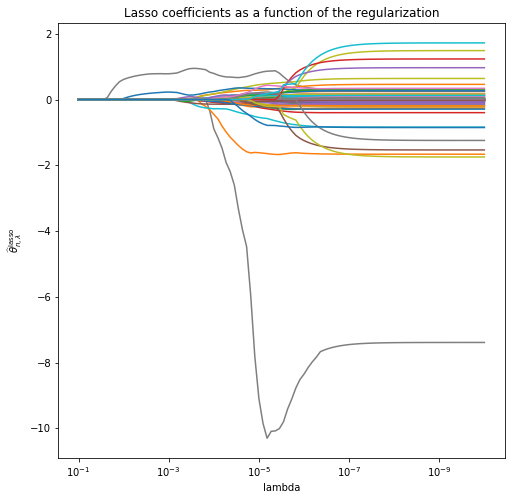
\includegraphics[width = .7\linewidth]{./Illustrations/lasso_coef.png}
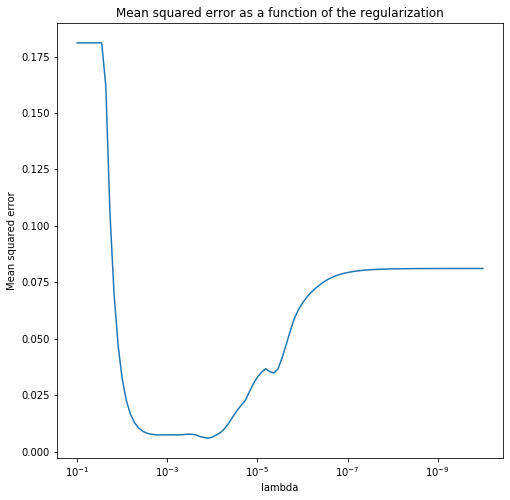
\includegraphics[width = .7\linewidth]{./Illustrations/lasso_rmse_test.png}
\end{center}
\caption{Lasso regression is used to predict the Brazilian inflation based on many observed variables, see \url{https://github.com/gabrielrvsc/HDeconometrics/}. The model is trained using $n=140$ data with for each $1\leqslant i \leqslant n$, $X_i\in\rset^{93}$, i.e. $d  =93$. The features are econometric data available each month. (Top) Estimated coefficient $\widehat \param^{\mathrm{lasso}}_{n,\lambda}$ as a function of $\lambda$. (Bottom) Mean squared error between the true observations and the predictions over the test set with $15$ new data points.}
\end{figure}


\begin{figure}
\begin{center}
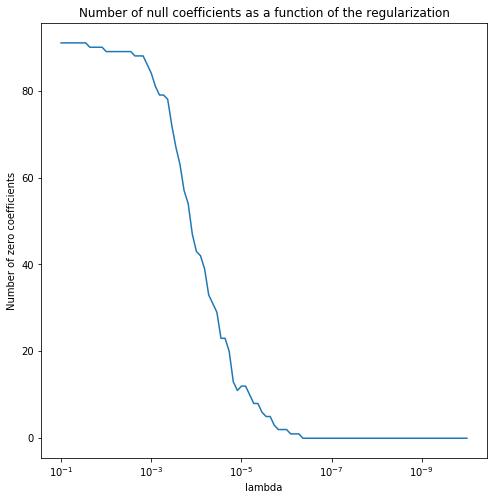
\includegraphics[width = .7\linewidth]{./Illustrations/lasso_nbzeros.png}
\end{center}
\caption{Lasso regression is used to predict the Brazilian inflation based on many observed variables, see \url{https://github.com/gabrielrvsc/HDeconometrics/}. The model is trained using $n=140$ data with for each $1\leqslant i \leqslant n$, $X_i\in\rset^{93}$, i.e. $d  =93$. The features are econometric data available each month. Number of null coefficient in $\widehat \param^{\mathrm{lasso}}_{n,\lambda}$ as a function of $\lambda$.}
\end{figure}
